\documentclass{article}
\usepackage{graphicx}
\usepackage{amsmath}
\usepackage{hyperref}
\usepackage{subcaption}
\usepackage{caption}


\graphicspath{{figures}}

\title{Paulownias: bipartite model trees for inductive interaction prediction}
\author{Pedro Ilídio}
\date{November 2024}

% name ideas: paulownia, catalpa, sycamore, maple
\begin{document}

\maketitle

\section{Methods}

\subsection{The Bipartite Global Single Output algorithm}
[TODO]

\subsection{Bipartite Model Trees}
\label{sec:bipartite-model-trees}
A decision tree represents a hierarchical clustering of the problem in hands. Their inference procedure corresponds to i) assigning the new incoming instance to one of the terminal clusters (the leaves); and then ii) returning the prototype of that cluster. Model trees differ from the traditional procedure in the second step. They consist of building a machine learning model for each terminal cluster, using only the training instances assigned to that cluster. After a test instance is assigned to a leaf, the prediction for that instance will be the output of that leaf's model. Notice that instances in the same leaf are thus allowed to yield distinct predictions, in contrast to the usual approach of returning a leaf-wise prototype.

For the present proposal, a simple distance-weighted nearest neighbors (DWNN) estimator is used as the leaf model. For a test instance $(x_\text{1, test},\; x_\text{2, test})$, the predicted probability $\tilde y$ of DWNN is given by
% todo: maybe explain the relationship with the bigger dyad-dyad kernel (kronecker product of d1 and d2)
%
\begin{equation}
    \label{eq:dwnn}
    \tilde y (x_\text{1, test},\; x_\text{2, test}) = 
        \frac{
            \sum_i\sum_j
            s(x_\text{1, test},\; X^i_\text{1, train})
            s(x_\text{2, test},\; X^j_\text{2, train})
            y^{ij}_\text{train}
        }{
            \sum_i\sum_j
            s(x_\text{1, test},\; X^i_\text{1, train})
            s(x_\text{2, test},\; X^j_\text{2, train})
        }
\end{equation}
%
in which $s(x_a,\; x_b)$ is an arbitrary similarity measure between instances $x_a$ and $x_b$. Since working with kernel matrices $\{\phi\}$ directly, we can also write
%
\begin{equation}
    \tilde y (x_\text{1, test},\; x_\text{2, test}) = 
        \frac{
            \sum_i\sum_j
            \phi^i_\text{1, test}
            \phi^j_\text{2, test}
            y^{ij}_\text{train}
        }{
            \sum_i\sum_j
            \phi^i_\text{1, test}
            \phi^j_\text{2, test}
        }\text{.}
\end{equation}

% A more general formulation would be to consider a dyad-dyad kernel $K = K(d_a, d_b)$:
To be explored in the following section, a more general formulation would be to consider a dyad-dyad kernel $K(d_a,\;d_b) = K[(x_{1a},\; x_{2a}),\; (x_{1b},\; x_{2b})]$:
%
\begin{equation}
    \label{eq:dyad-dyad}
    \tilde y (x_\text{1, test},\; x_\text{2, test}) = 
        \frac{
            \sum_i\sum_j
            K[(x_\text{1, test},\; X^i_\text{1, train}),\; (x_\text{2, test},\; X^j_\text{2, train})]
            y^{ij}_\text{train}
        }{
            \sum_i\sum_j
            K[(x_\text{1, test},\; X^i_\text{1, train}),\; (x_\text{2, test},\; X^j_\text{2, train})]
        }\text{.}
\end{equation}

In our specific case, we set $K[(x_{1a},\; x_{2a}),\; (x_{1b},\; x_{2b})] = s(x_{1a},\; x_{1b})s(x_{2a},\; x_{2b})$.

[Maybe I should start with the more general formulation?]

[WIP]

In matrix notation, the predictions $\tilde Y$ can be written as
%
%This formulation corresponds to a more 
\begin{equation}  % Wrong!
    \tilde Y = 
        \frac{(\Phi_1 \otimes \Phi_2)
        vec(Y_\text{train})}{(\Phi_1 \odot \Phi_2)}
        =
        \frac{(\Phi_1 Y_\text{train} \Phi_2)
        }{(\Phi_1 \odot \Phi_2)}
\end{equation}


\section{Motivation}
\subsection{Paulownias inference is a generalization of the inference procedure of PBCTs}

% todo: performance improves
In the original description of PBCTs, \cite{pliakos2018} proposed a variant of the inference procedure for the cases in which one of the instances of the dyad is present in the training set. Remember that each leaf of a PBCT will correspond to a 2D partition $Y_\text{leaf}$ of the training interaction matrix. In the variant proposed by \cite{pliakos2018}, if the test row instance is known, the output will be the average of only the row corresponding to that instance, and not over the entire $Y_\text{leaf}$ as usual. This is done analogously for a known column instance as well. In precise terms, the predicted probability $\tilde y$ for a test instance $(x_\text{1, test}, x_\text{2, test})$ is given by \autoref{eq:pbct}, in which $\mathcal{I}_\text{leaf}$ and $\mathcal{J}_\text{leaf}$ are the sets of row and column indices in the leaf, respectively.
%
\begin{equation}
    \label{eq:pbct}
    \tilde y (x_\text{1, test},\; x_\text{2, test}) = \begin{cases}
        \frac{1}{|\mathcal{J}_\text{leaf}|} \sum_{j \in \mathcal{J}_\text{leaf}} y^{ij}_\text{train} & \text{if } \exists \; i : x_\text{1, test} = X^i_\text{1, train} \\        
        \frac{1}{|\mathcal{I}_\text{leaf}|} \sum_{i \in \mathcal{I}_\text{leaf}} y^{ij}_\text{train} & \text{if } \exists\; j : x_\text{2, test} = X^j_\text{2, train} \\
        \frac{1}{|\mathcal{I}_\text{leaf}||\mathcal{J}_\text{leaf}|} \sum_{i \in \mathcal{I}_\text{leaf}}\sum_{j \in \mathcal{J}_\text{leaf}} y^{ij}_\text{train} & \text{otherwise.}\\
    \end{cases}
\end{equation}
%
If we define $\mathbb{I}(\cdot)$ as the binary indicator function
\begin{equation}
    \mathbb{I}(A) = \begin{cases}
        1 & \text{if A is true} \\
        0 & \text{otherwise},
    \end{cases}
\end{equation}
%
% and set $s(x_a,\;  x_b) = \mathbb{I}(x_a = x_b)$, \autoref{eq:pbct} is equivalent to \autoref{eq:dwnn}. [FIXME: blatanly wrong]
and set $K(d_a,\; d_b) = \mathbb{I}(x_{1a} = x_{1b}) + \mathbb{I}(x_{1a} = x_{1b})$, \ref{eq:pbct} is equivalent to \ref{eq:dyad-dyad}.
Specifically for kernel matrices, we have that $\phi_1^i = s(x_\text{1, test},\; X^i_\text{1, train})$, so $x_\text{1, test} = X^i_\text{1, train} \iff \phi_1^i = 1$ and therefore \autoref{eq:pbct} can be written as
%
\begin{equation}
    \tilde y (x_\text{1, test},\; x_\text{2, test}) = 
        \frac{
            \sum_i\sum_j
            [
                \mathbb{I}(\phi^i_\text{1, test} = 1)
                +              
                \mathbb{I}(\phi^j_\text{2, test} = 1)
            ]
            y^{ij}_\text{train}
        }{
            \sum_i\sum_j
            [
                \mathbb{I}(\phi^i_\text{1, test} = 1)
                +              
                \mathbb{I}(\phi^j_\text{2, test} = 1)
            ]
        }\text{.}
\end{equation}


This inference procedure is attributed as default to the Global Multi-Output trees (GMO) introduced by \citetext{pliakos2018}, while averaging all the values in $Y_\text{leaf}$ ($K(\cdot)=1$) is denoted GMO with single-label average (GMOsa) by the same authors. A visual comparison of the inference procedures using the GMO, GMOsa and the DWNN strategies is depicted in \autoref{fig:procedure}.

\begin{figure}
    \centering
    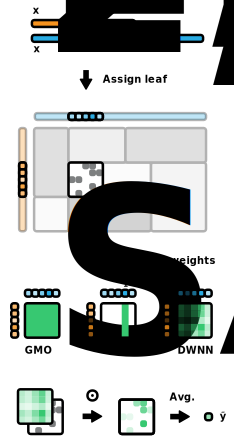
\includegraphics[width=.7\textwidth]{procedure}
    \caption{Depiction of the inference procedure of a bipartite decision tree, visualy comparing GMO, GMOsa and the DWNN strategies for determining the final output value from the leaf partition.}
    \label{fig:procedure}
\end{figure}

The proposed approach (\autoref{sec:bipartite-model-trees}) places itself as a middle ground between the two extremes. We still utilize all the annotations in the leaf, while also still prioritizing similar instances when generating the final prediction. Therefore, we offer a more flexible framework to fine-tune biclustering decision trees along the bias-variance spectrum.

[ours work for DWNN]
[add a more tangible example in which the original PBCT inference would not be ideal]

\section{Experimental setup}
[less finished ideas]

In fact, a main rationale behind model trees is to combine a simple high-bias model (such as linear regression) with the high-variance and low-bias decision trees, balancing their respective strengths and weaknesses. While the simple models are commonly unsufficient to represent the data as a whole, they often provide good local approximations to the learning task. Using a decision tree allows these models to be applied separately to specific regions of the feature space, in a similar fashion to how a non-linear function can often be locally approximated by a linear one.

% TODO: Another benefit would be in terms of computational complexity...

However, two trivial explanations must be ruled out for the hypothesized benefits to hold and for the proposed approach to be justifiable:
%
\begin{enumerate}
    \item \textbf{The leaf model is doing all the work:} the simple model is already able to capture the underlying patterns in the data, and the tree partitioning is not adding any value to the model.
    \item \textbf{Large leaves are enough:} setting the leaf size to be large enough would already provide the same benefits as the proposed approach. This corresponds to setting the leaf model to the simplest possible estimator: the label average.
    % \item \textbf{The specific weights are irrelevant:} the distance-based weighting procedure is not adding any value to the model, and the same results could be achieved by using random weights in the leaves. [this is hard to explain, I think it has some reason but I still have to think it through]
\end{enumerate}

[the experiments will be designed in the direction of ruling out these explanations]

\section{Results and discussion}

\subsection{Paulownias outperform previous methods for inductive interaction prediction}

\begin{figure}
    \centering
    \begin{subfigure}{.24\textwidth}
        \includegraphics[width=\textwidth]{results/literature_methods/TT/all_datasets/boxplots/TT__auroc.pdf}
    \end{subfigure}
    \begin{subfigure}{.24\textwidth}
        \includegraphics[width=\textwidth]{results/literature_methods/TT_25/all_datasets/boxplots/TT__auroc.pdf}
    \end{subfigure}
    \begin{subfigure}{.24\textwidth}
        \includegraphics[width=\textwidth]{results/literature_methods/TT_50/all_datasets/boxplots/TT__auroc.pdf}
    \end{subfigure}
    \begin{subfigure}{.24\textwidth}
        \includegraphics[width=\textwidth]{results/literature_methods/TT_75/all_datasets/boxplots/TT__auroc.pdf}
    \end{subfigure}

     \begin{subfigure}{.24\textwidth}
        \includegraphics[width=\textwidth]{results/literature_methods/TT/all_datasets/boxplots/TT__auprc.pdf}
    \end{subfigure}
    \begin{subfigure}{.24\textwidth}
        \includegraphics[width=\textwidth]{results/literature_methods/TT_25/all_datasets/boxplots/TT__auprc.pdf}
    \end{subfigure}
    \begin{subfigure}{.24\textwidth}
        \includegraphics[width=\textwidth]{results/literature_methods/TT_50/all_datasets/boxplots/TT__auprc.pdf}
    \end{subfigure}
    \begin{subfigure}{.24\textwidth}
        \includegraphics[width=\textwidth]{results/literature_methods/TT_75/all_datasets/boxplots/TT__auprc.pdf}
    \end{subfigure}   
    \caption{Performance comparison of the proposed Paulownias with the previous methods for inductive interaction prediction.}
    \label{fig:literature_TT}
\end{figure}

\begin{figure}
    \centering
    \begin{subfigure}{.24\textwidth}
        \includegraphics[width=\textwidth]{results/literature_methods/TT/all_datasets/boxplots/LT+TL__auroc.pdf}
    \end{subfigure}
    \begin{subfigure}{.24\textwidth}
        \includegraphics[width=\textwidth]{results/literature_methods/TT_25/all_datasets/boxplots/LT+TL__auroc.pdf}
    \end{subfigure}
    \begin{subfigure}{.24\textwidth}
        \includegraphics[width=\textwidth]{results/literature_methods/TT_50/all_datasets/boxplots/LT+TL__auroc.pdf}
    \end{subfigure}
    \begin{subfigure}{.24\textwidth}
        \includegraphics[width=\textwidth]{results/literature_methods/TT_75/all_datasets/boxplots/LT+TL__auroc.pdf}
    \end{subfigure}

     \begin{subfigure}{.24\textwidth}
        \includegraphics[width=\textwidth]{results/literature_methods/TT/all_datasets/boxplots/LT+TL__auprc.pdf}
    \end{subfigure}
    \begin{subfigure}{.24\textwidth}
        \includegraphics[width=\textwidth]{results/literature_methods/TT_25/all_datasets/boxplots/LT+TL__auprc.pdf}
    \end{subfigure}
    \begin{subfigure}{.24\textwidth}
        \includegraphics[width=\textwidth]{results/literature_methods/TT_50/all_datasets/boxplots/LT+TL__auprc.pdf}
    \end{subfigure}
    \begin{subfigure}{.24\textwidth}
        \includegraphics[width=\textwidth]{results/literature_methods/TT_75/all_datasets/boxplots/LT+TL__auprc.pdf}
    \end{subfigure}   
    \caption{Performance comparison of the proposed Paulownias with the previous methods for inductive interaction prediction.}
    \label{fig:literature_LTTL}
\end{figure}


\subsection{Using similarities with neighbors is the best way of generating outputs}

\begin{figure}
    \centering
    \begin{subfigure}{.24\textwidth}
        \includegraphics[width=\textwidth]{results/dwnn_weights/TT/all_datasets/boxplots/TT__auroc.pdf}
    \end{subfigure}
    \begin{subfigure}{.24\textwidth}
        \includegraphics[width=\textwidth]{results/dwnn_weights/TT_25/all_datasets/boxplots/TT__auroc.pdf}
    \end{subfigure}
    \begin{subfigure}{.24\textwidth}
        \includegraphics[width=\textwidth]{results/dwnn_weights/TT_50/all_datasets/boxplots/TT__auroc.pdf}
    \end{subfigure}
    \begin{subfigure}{.24\textwidth}
        \includegraphics[width=\textwidth]{results/dwnn_weights/TT_75/all_datasets/boxplots/TT__auroc.pdf}
    \end{subfigure}

     \begin{subfigure}{.24\textwidth}
        \includegraphics[width=\textwidth]{results/dwnn_weights/TT/all_datasets/boxplots/TT__auprc.pdf}
    \end{subfigure}
    \begin{subfigure}{.24\textwidth}
        \includegraphics[width=\textwidth]{results/dwnn_weights/TT_25/all_datasets/boxplots/TT__auprc.pdf}
    \end{subfigure}
    \begin{subfigure}{.24\textwidth}
        \includegraphics[width=\textwidth]{results/dwnn_weights/TT_50/all_datasets/boxplots/TT__auprc.pdf}
    \end{subfigure}
    \begin{subfigure}{.24\textwidth}
        \includegraphics[width=\textwidth]{results/dwnn_weights/TT_75/all_datasets/boxplots/TT__auprc.pdf}
    \end{subfigure}   
    \caption{Performance comparison of the proposed Paulownias with the previous methods for inductive interaction prediction.}
    \label{fig:weights_TT}
\end{figure}

\begin{figure}
    \centering
    \begin{subfigure}{.24\textwidth}
        \includegraphics[width=\textwidth]{results/dwnn_weights/TT/all_datasets/boxplots/LT+TL__auroc.pdf}
    \end{subfigure}
    \begin{subfigure}{.24\textwidth}
        \includegraphics[width=\textwidth]{results/dwnn_weights/TT_25/all_datasets/boxplots/LT+TL__auroc.pdf}
    \end{subfigure}
    \begin{subfigure}{.24\textwidth}
        \includegraphics[width=\textwidth]{results/dwnn_weights/TT_50/all_datasets/boxplots/LT+TL__auroc.pdf}
    \end{subfigure}
    \begin{subfigure}{.24\textwidth}
        \includegraphics[width=\textwidth]{results/dwnn_weights/TT_75/all_datasets/boxplots/LT+TL__auroc.pdf}
    \end{subfigure}

     \begin{subfigure}{.24\textwidth}
        \includegraphics[width=\textwidth]{results/dwnn_weights/TT/all_datasets/boxplots/LT+TL__auprc.pdf}
    \end{subfigure}
    \begin{subfigure}{.24\textwidth}
        \includegraphics[width=\textwidth]{results/dwnn_weights/TT_25/all_datasets/boxplots/LT+TL__auprc.pdf}
    \end{subfigure}
    \begin{subfigure}{.24\textwidth}
        \includegraphics[width=\textwidth]{results/dwnn_weights/TT_50/all_datasets/boxplots/LT+TL__auprc.pdf}
    \end{subfigure}
    \begin{subfigure}{.24\textwidth}
        \includegraphics[width=\textwidth]{results/dwnn_weights/TT_75/all_datasets/boxplots/LT+TL__auprc.pdf}
    \end{subfigure}   
    \caption{Performance comparison of the proposed Paulownias with the previous methods for inductive interaction prediction.}
    \label{fig:weights_LTTL}
\end{figure}

\subsection{Larger leaves are not enough to explain the performance improvement}

\subsection{Semi-supervised impurities do not offer significant advantage to Paulownias}

\subsection{Matrix completion slightly improves predictive performance}

\begin{figure}
    \centering
    \begin{subfigure}{.24\textwidth}
        \includegraphics[width=\textwidth]{results/y_reconstruction/TT/all_datasets/boxplots/TT__auroc.pdf}
    \end{subfigure}
    \begin{subfigure}{.24\textwidth}
        \includegraphics[width=\textwidth]{results/y_reconstruction/TT_25/all_datasets/boxplots/TT__auroc.pdf}
    \end{subfigure}
    \begin{subfigure}{.24\textwidth}
        \includegraphics[width=\textwidth]{results/y_reconstruction/TT_50/all_datasets/boxplots/TT__auroc.pdf}
    \end{subfigure}
    \begin{subfigure}{.24\textwidth}
        \includegraphics[width=\textwidth]{results/y_reconstruction/TT_75/all_datasets/boxplots/TT__auroc.pdf}
    \end{subfigure}

     \begin{subfigure}{.24\textwidth}
        \includegraphics[width=\textwidth]{results/y_reconstruction/TT/all_datasets/boxplots/TT__auprc.pdf}
    \end{subfigure}
    \begin{subfigure}{.24\textwidth}
        \includegraphics[width=\textwidth]{results/y_reconstruction/TT_25/all_datasets/boxplots/TT__auprc.pdf}
    \end{subfigure}
    \begin{subfigure}{.24\textwidth}
        \includegraphics[width=\textwidth]{results/y_reconstruction/TT_50/all_datasets/boxplots/TT__auprc.pdf}
    \end{subfigure}
    \begin{subfigure}{.24\textwidth}
        \includegraphics[width=\textwidth]{results/y_reconstruction/TT_75/all_datasets/boxplots/TT__auprc.pdf}
    \end{subfigure}   
    \caption{Performance comparison of the proposed Paulownias with the previous methods for inductive interaction prediction.}
    \label{fig:ss_TT}
\end{figure}

\begin{figure}
    \centering
    \begin{subfigure}{.24\textwidth}
        \includegraphics[width=\textwidth]{results/y_reconstruction/TT/all_datasets/boxplots/LT+TL__auroc.pdf}
    \end{subfigure}
    \begin{subfigure}{.24\textwidth}
        \includegraphics[width=\textwidth]{results/y_reconstruction/TT_25/all_datasets/boxplots/LT+TL__auroc.pdf}
    \end{subfigure}
    \begin{subfigure}{.24\textwidth}
        \includegraphics[width=\textwidth]{results/y_reconstruction/TT_50/all_datasets/boxplots/LT+TL__auroc.pdf}
    \end{subfigure}
    \begin{subfigure}{.24\textwidth}
        \includegraphics[width=\textwidth]{results/y_reconstruction/TT_75/all_datasets/boxplots/LT+TL__auroc.pdf}
    \end{subfigure}

     \begin{subfigure}{.24\textwidth}
        \includegraphics[width=\textwidth]{results/y_reconstruction/TT/all_datasets/boxplots/LT+TL__auprc.pdf}
    \end{subfigure}
    \begin{subfigure}{.24\textwidth}
        \includegraphics[width=\textwidth]{results/y_reconstruction/TT_25/all_datasets/boxplots/LT+TL__auprc.pdf}
    \end{subfigure}
    \begin{subfigure}{.24\textwidth}
        \includegraphics[width=\textwidth]{results/y_reconstruction/TT_50/all_datasets/boxplots/LT+TL__auprc.pdf}
    \end{subfigure}
    \begin{subfigure}{.24\textwidth}
        \includegraphics[width=\textwidth]{results/y_reconstruction/TT_75/all_datasets/boxplots/LT+TL__auprc.pdf}
    \end{subfigure}   
    \caption{Performance comparison of the proposed Paulownias with the previous methods for inductive interaction prediction.}
    \label{fig:ss_LTTL}
\end{figure}

% Another possible explanation for the superiority of the proposed approach is that the weighting procedure captures the underlying missingness mechanism.
% In other words, the weighting corresponds to more distant features tend increases diversity between trees in an ensemble.


% Mitigate the effect of distant negative annotations

% possible explanations
% big leafs may already do the job
% the leaf model is doing all the work
%   we must use it as a baseline
% indirect weighting by node size:
%   random "similarities" would still do the job
%   consider leaf size when averaging trees in a forest (use RandomForestClassifier instead of RandomForestRegressor).

%
% \begin{equation}
% s(x_a,\;  x_b) = \mathbb{I}(x_a = x_b)
% \end{equation}
%
%
% \begin{equation}
%     \tilde y (x_\text{1, test}, x_\text{2, test}) = 
%         \frac{
%             \sum_{i \in \mathcal{I}_\text{leaf}}\sum_{j \in \mathcal{J}_\text{leaf}}
%             w^{ij}(x_\text{1, test}, x_\text{2, test})
%             y^{ij}_\text{train}
%         }{
%             \sum_{i \in \mathcal{I}_\text{leaf}}\sum_{j \in \mathcal{J}_\text{leaf}}
%             w^{ij}(x_\text{1, test}, x_\text{2, test})
%         }
% \end{equation}
% \begin{equation}
%     \tilde y (x_\text{1, test}, x_\text{2, test}) = 
%         \frac{
%             \sum_{i \in \mathcal{I}_\text{leaf}}\sum_{j \in \mathcal{J}_\text{leaf}}
%             \mathbb{I}(x_\text{1, test} = X^i_\text{1, train})
%             \mathbb{I}(x_\text{2, test} = X^j_\text{2, train})
%             y^{ij}_\text{train}
%         }{
%             \sum_{i \in \mathcal{I}_\text{leaf}}\sum_{j \in \mathcal{J}_\text{leaf}}
%             \mathbb{I}(x_\text{1, test} = X^i_\text{1, train})
%             \mathbb{I}(x_\text{2, test} = X^j_\text{2, train})
%         }
% \end{equation}

%When working with pairwise similarities, $x_\text{1, test} = X^î_\text{train} \iff x^i_\text{1, test} = 1$. Therefore,
%%
%\begin{equation}
%w^{ij}(x_\text{1, test}, x_\text{2, test}) =
%    \mathbb{I}(x_\text{1, test} = X^i_\text{1, train}) \mathbb{I}(x_\text{2, test} = X^j_\text{2, train})
%\end{equation}
%
%Under this formulation, a natural extension would be


% TODO experiments:
% big-leaf PBCT

\end{document}
